

%----------------------------------------------------------------------------------------
%	PACKAGES AND OTHER DOCUMENT CONFIGURATIONS
%----------------------------------------------------------------------------------------

\documentclass{article}

\usepackage{fancyhdr} % Required for custom headers
\usepackage{lastpage} % Required to determine the last page for the footer
\usepackage{extramarks} % Required for headers and footers
\usepackage[usenames,dvipsnames]{color} % Required for custom colors
\usepackage{graphicx} % Required to insert images
\usepackage{listings} % Required for insertion of code
\usepackage{courier} % Required for the courier font


% Margins
\topmargin=-0.45in
\evensidemargin=0in
\oddsidemargin=0in
\textwidth=6.5in
\textheight=9.0in
\headsep=0.25in

\linespread{1.1} % Line spacing

% Set up the header and footer
\pagestyle{fancy}
\lhead{\hmwkAuthorName\ : \hmwkStudentID} % Top left header
\chead{ \hmwkClassShort} % Top center head
\rhead{\firstxmark} % Top right header
\lfoot{\lastxmark} % Bottom left footer
\cfoot{} % Bottom center footer
\rfoot{Page\ \thepage\ of\ \protect\pageref{LastPage}} % Bottom right footer
\renewcommand\headrulewidth{0.4pt} % Size of the header rule
\renewcommand\footrulewidth{0.4pt} % Size of the footer rule

\setlength\parindent{0pt} % Removes all indentation from paragraphs

%----------------------------------------------------------------------------------------
%	CODE INCLUSION CONFIGURATION
%----------------------------------------------------------------------------------------

\definecolor{MyDarkGreen}{rgb}{0.0,0.4,0.0} % This is the color used for comments
\lstloadlanguages{C} % Load Perl syntax for listings, for a list of other languages supported see: ftp://ftp.tex.ac.uk/tex-archive/macros/latex/contrib/listings/listings.pdf
\lstset{language=C, % Use c in this example
        frame=single, % Single frame around code
        basicstyle=\small\ttfamily, % Use small true type font
        keywordstyle=[1]\color{Blue}\bf, % cfunctions bold and blue
        keywordstyle=[2]\color{Purple}, % c function arguments purple
        keywordstyle=[3]\color{Blue}\underbar, % Custom functions underlined and blue
        identifierstyle=, % Nothing special about identifiers                                         
        commentstyle=\usefont{T1}{pcr}{m}{sl}\color{MyDarkGreen}\small, % Comments small dark green courier font
        stringstyle=\color{Purple}, % Strings are purple
        showstringspaces=false, % Don't put marks in string spaces
        tabsize=5, % 5 spaces per tab
        %
        % Put standard c functions not included in the default language here
        morekeywords={rand},
        %
        % Put c function parameters here
        morekeywords=[2]{on, off, interp},
        %
        % Put user defined functions here
        morekeywords=[3]{test},
       	%
        morecomment=[l][\color{Blue}]{...}, % Line continuation (...) like blue comment
        numbers=left, % Line numbers on left
        firstnumber=1, % Line numbers start with line 1
        numberstyle=\tiny\color{Blue}, % Line numbers are blue and small
        stepnumber=1 % Line numbers go in steps of 5
}

% Creates a new command to include a script, the first parameter is the filename of the script (without .txt), the second parameter is the caption
\newcommand{\Cscript}[2]{
\begin{itemize}
\item[]\lstinputlisting[caption=#2,label=#1]{#1.txt}
\end{itemize}
}

%----------------------------------------------------------------------------------------
%	DOCUMENT STRUCTURE COMMANDS
%	Skip this unless you know what you're doing
%----------------------------------------------------------------------------------------

% Header and footer for when a page split occurs within a problem environment
\newcommand{\enterProblemHeader}[1]{
\nobreak\extramarks{#1}{#1 continued on next page\ldots}\nobreak
\nobreak\extramarks{#1 }{#1 continued on next page\ldots}\nobreak
}

% Header and footer for when a page split occurs between problem environments
\newcommand{\exitProblemHeader}[1]{
\nobreak\extramarks{#1}{#1 continued on next page\ldots}\nobreak
\nobreak\extramarks{#1}{}\nobreak
}

\setcounter{secnumdepth}{0} % Removes default section numbers
\newcounter{homeworkProblemCounter} % Creates a counter to keep track of the number of problems

\newcommand{\homeworkProblemName}{}
\newenvironment{homeworkProblem}[1][Problem \arabic{homeworkProblemCounter}]{ % Makes a new environment called homeworkProblem which takes 1 argument (custom name) but the default is "Problem #"
\stepcounter{homeworkProblemCounter} % Increase counter for number of problems
\renewcommand{\homeworkProblemName}{#1} % Assign \homeworkProblemName the name of the problem
\section{\homeworkProblemName} % Make a section in the document with the custom problem count
\enterProblemHeader{\homeworkProblemName} % Header and footer within the environment
}{
\exitProblemHeader{\homeworkProblemName} % Header and footer after the environment
}

\newcommand{\problemAnswer}[1]{ % Defines the problem answer command with the content as the only argument
\noindent\framebox[\columnwidth][c]{\begin{minipage}{0.98\columnwidth}#1\end{minipage}} % Makes the box around the problem answer and puts the content inside
}

\newcommand{\homeworkSectionName}{}
\newenvironment{homeworkSection}[1]{ % New environment for sections within homework problems, takes 1 argument - the name of the section
\renewcommand{\homeworkSectionName}{#1} % Assign \homeworkSectionName to the name of the section from the environment argument
\subsection{\homeworkSectionName} % Make a subsection with the custom name of the subsection
\enterProblemHeader{\homeworkProblemName} % Header and footer within the environment
}{
\enterProblemHeader{\homeworkProblemName} % Header and footer after the environment
}

%----------------------------------------------------------------------------------------
%	NAME AND CLASS SECTION
%----------------------------------------------------------------------------------------

\newcommand{\hmwkTitle}{207SE Operating Systems, Security and Networks Portfolio} % Assignment title
\newcommand{\hmwkDueDate}{Monday,\ December\ 15th,\ 2014} % Due date
\newcommand{\hmwkClass}{ECU178 \- Computer Science} % Course/class
\newcommand{\hmwkClassTime}{10:30am} % Class/lecture time
\newcommand{\hmwkClassInstructor}{Dr Mark Elshaw} % Teacher/lecturer
\newcommand{\hmwkAuthorName}{Robert Rigler} % Your name
\newcommand{\hmwkStudentID}{4939377}% My Student ID
\newcommand{\hmwkClassShort}{207SE Portfolio} %Short name for class (only used in header)

%----------------------------------------------------------------------------------------
%	TITLE PAGE
%----------------------------------------------------------------------------------------

\title{
\vspace{2in}
\textmd{\textbf{\hmwkClass:\ \\ \hmwkTitle}}\\
\normalsize\vspace{0.1in}\small{Due\ on\ \hmwkDueDate}\\
\vspace{0.1in}\large{\textit{\hmwkClassInstructor\ }}
\vspace{3in}
}

\author{\textbf{\hmwkAuthorName\ : \hmwkStudentID}}
\date{} % Insert date here if you want it to appear below your name

%----------------------------------------------------------------------------------------

\begin{document}

\maketitle

%----------------------------------------------------------------------------------------
%	TABLE OF CONTENTS
%----------------------------------------------------------------------------------------

%\setcounter{tocdepth}{1} % Uncomment this line if you don't want subsections listed in the ToC

\newpage
\tableofcontents
\newpage

%----------------------------------------------------------------------------------------
%	PROBLEM 1
%----------------------------------------------------------------------------------------

% To have just one problem per page, simply put a \clearpage after each problem

\begin{homeworkProblem}[Item 1 - Linux Command Line]{}
\homeworkSection{1. Make home directory read/write/executable only for myself}
\begin{enumerate}

\item Linux Command: chmod u+rwx ~/ \\
\begin{center}
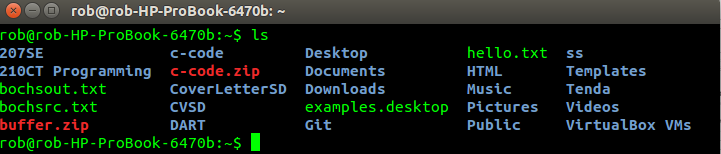
\includegraphics[width=0.9\columnwidth]{Assignment_1/l1.png}
\end{center}
\end{enumerate}

\homeworkSection{2. Download the script from http://www.centerkey.com/tree/tree.sh and make it executable}
\begin{enumerate}
\item Linux Command: wget http://www.centerkey.com/tree/tree.sh
\item Linux Command: chmod 700 tree.sh
\begin{center}
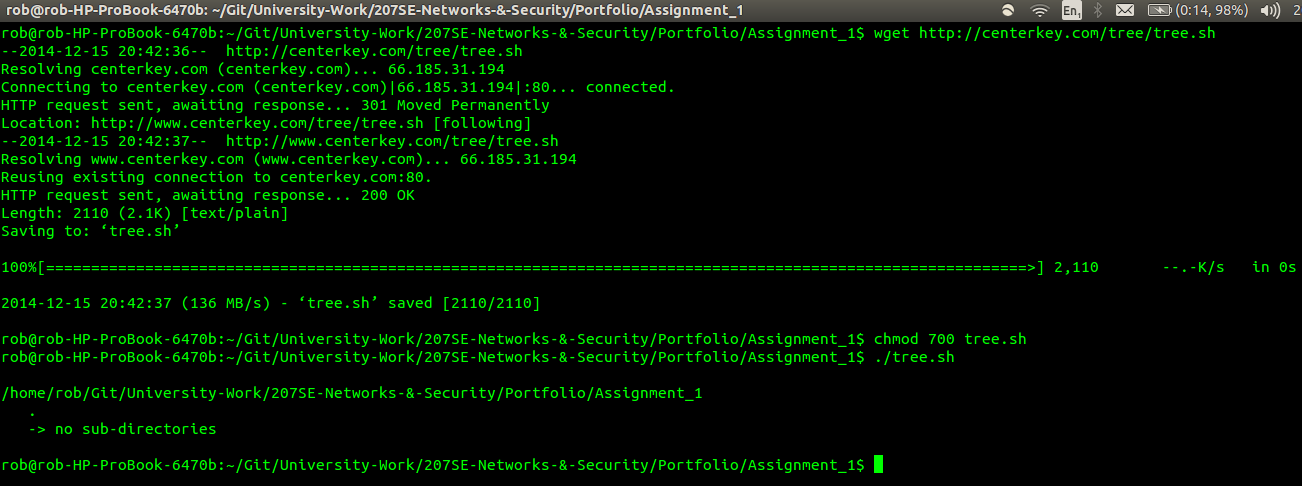
\includegraphics[width=0.9\columnwidth]{Assignment_1/l2.png}
\end{center}
\end{enumerate}

\homeworkSection{3. Making Directories}
\begin{enumerate}
\item Making a directory called 207SE in Home folder \\
Linux Command: mkdir 207SE
\item Create sub-directory called Portfolio\\
Linux Command: mkdir Portfolio
\item Create numbered directories from week 1 and week 2\\
Linux Command: mkdir 1\\
Linux Command: mkdir 2
\item Transfer work from week 1 into the folder called 1\\
Linux Command: mv HarvardArchitecture.txt ~/207SE/Portfolio/1
\item Evidence of directory using tree.sh

\begin{center}
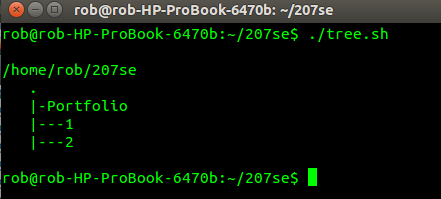
\includegraphics[width=0.9\columnwidth]{Assignment_1/l3.png}
\end{center}
\end{enumerate}

\homeworkSection{4. Display who is logged on and sort them in alphabetical order}
\begin{enumerate}
\item Linux Command: who | sort
\item Evidence of output:
\begin{center}
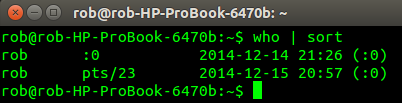
\includegraphics[width=0.9\columnwidth]{Assignment_1/l4.png}
\end{center}
\end{enumerate}

\homeworkSection{5. Talk, Write and Wall}
\begin{enumerate}
\item Write: Writes what the user types to the terminal of another specified user.
\item Talk: Opens a two-way conversation using a terminal
\item Wall: displays a message to all users on the system
\end{enumerate}

\homeworkSection{6. Stop bugging me}
\begin{enumerate}
\item 'mesg n' Will stop write, wall and talk from interrupting the user.
\end{enumerate}

\homeworkSection{7. Find the number of words and lines in poem.txt}
\begin{enumerate}
\item Linux Command. wc poem.txt\\
 Evidence of output: 
\begin{center}
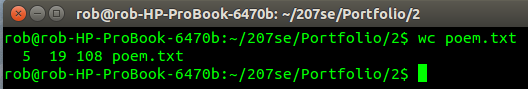
\includegraphics[width=0.9\columnwidth]{Assignment_1/l5.png}
\end{center}
\end{enumerate}
\homeworkSection{8. Grep the lines containing 'and' and the number of lines}

\begin{enumerate}
\item Linux Command: grep -n 'and' poem.txt\\
Evidence of Output: 
\begin{center}
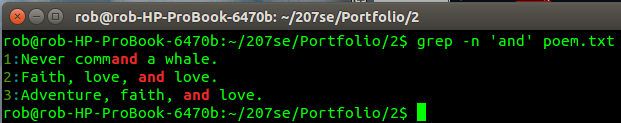
\includegraphics[width=0.9\columnwidth]{Assignment_1/l6.png}
\end{center}
\end{enumerate}


\homeworkSection{9. Use cat to display the contents of the file}
\begin{enumerate}
\item Linux Command: cat poem.txt\\
Evidence of Output: 
\begin{center}
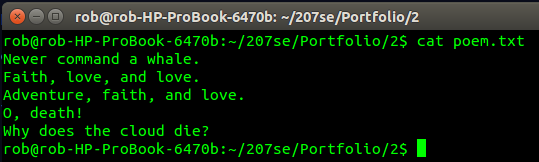
\includegraphics[width=0.9\columnwidth]{Assignment_1/l7.png}
\end{center}
\end{enumerate}

\homeworkSection{10. Sort the contents of poem.txt and redirect the output to poem2.txt}
\begin{enumerate}
\item Linux Command: sort poem.txt \textgreater poem2.txt\\
Evidence of Output: 
\begin{center}
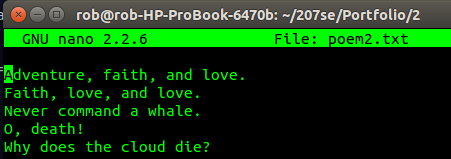
\includegraphics[width=0.9\columnwidth]{Assignment_1/l8.png}
\end{center}
\end{enumerate}

\homeworkSection{11. Sort the contents of poem.txt, reverse it, and then redirect the output to poem2.txt}
\begin{enumerate}
\item Linux Command: sort poem.txt | rev \textgreater poem2.txt\\
Evidence of Output: 
\begin{center}
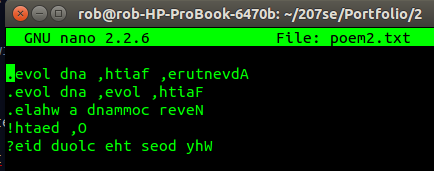
\includegraphics[width=0.9\columnwidth]{Assignment_1/l9.png}
\end{center}
\end{enumerate}

\end{homeworkProblem}
\clearpage

%----------------------------------------------------------------------------------------
%	PROBLEM 2
%----------------------------------------------------------------------------------------

\begin{homeworkProblem}[Item 2 - Assembly Code]
\begin{homeworkSection}{1. Right-Angled triangle}
The aim of this task was to produce a right-angled triangle of height specified by the user.\\
The process outline for this task is quite simple:
\begin{enumerate}
\item Get the user input and assign that value to the ecx register
\item Start the outer loop, then push the outerLoop value to the stack and move the innerLoop value into ecx.
\item Start the InnerLoop and print the '*' character the number of times specified in ecx.
\item After the InnerLoop is finished, start a new line and pop the OuterLoop value off of the stack.
\item Increment the InnerLoop value by 1 (So that one more triangle is draw next iteration) and repeat the Outerloop with the value in the ecx register (which is automatically decremented by one each time the Outerloop is called).
\end{enumerate}
 
\Cscript{Assignment_2/t1/rat}{Right angled triangle}
\problemAnswer{

\begin{center}
\large{Evidence of Right angled triangle}\vspace{5mm}
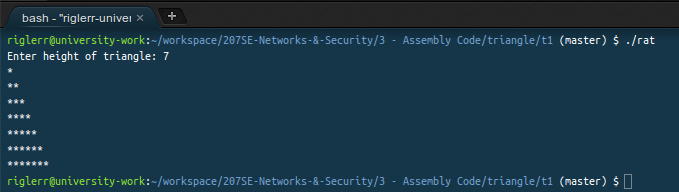
\includegraphics[width=0.9\columnwidth]{Assignment_2/t1/Evi1.png} 
\end{center}

}
\clearpage
\end{homeworkSection}
\begin{homeworkSection}{2. Isosceles Triangle}
The process to draw this triangle is similar to the previous task, but an additional loop is needed to print the required number of spaces before drawing the asterisks.
\begin{enumerate}
\item Get the user input for the height of the triangle and place it in the ecx register.
\item Work out the width of the triangle using the formula $2h-1$ where \emph{h} is the height specified by the user, and place this value in a variable called height.
\item Start the outerLoop and push its value to the stack.
\item Calculate the number of spaces that need to be drawn using the formula $(width-noOfAsterisks)/2$. The noOfAsterisks is the current value of the innerLoop (which is always an odd number). And place that value in ecx to be used as the control value for the third loop.
\item When dividing the value of $(width-noOfAsterisks)$ by 2, if the value is zero(on the last line), then do not print any spaces.
\item Draw spaces ecx times.
\item Pop innerLoop value of off stack and start innerLoop.
\item Start a new line, add 2 to the value of the innerLoop (The number of stars in each line increases by two each time.
\item Pop the value of the outerLoop off of the stack and start the next iteration.
\end{enumerate}
\Cscript{Assignment_2/t2/iso}{Isosceles Triangle Code}
\problemAnswer{

\begin{center}
\large{Evidence of triangle}\vspace{5mm}
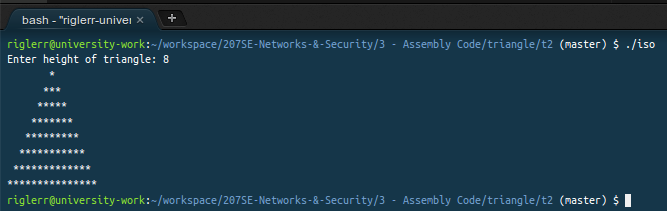
\includegraphics[width=0.9\columnwidth]{Assignment_2/t2/Evi1.png} 
\end{center}

}


\end{homeworkSection}

\end{homeworkProblem}
\clearpage
%----------------------------------------------------------------------------------------
%	PROBLEM 3
%----------------------------------------------------------------------------------------
\begin{homeworkProblem}[Item 3 - Bootloader]{}
This tasks was to create a bootloader using Assembly and boot into this bootloader using bochs.
The process involved:
\begin{enumerate}
\item Writing and compiling the code.
\item Writing the code to the first 512 bytes of a bootable image.
\item use bochs to run the bootloader.

\end{enumerate} 

\begin{homeworkSection}{1. Boot pragma-linux using bochs}
I created a Bash script to compile, create and simulate the bootloader.
\Cscript{Assignment_3/Task0/script}{Bash Script }
\clearpage
\begin{center}
\large{Evidence of bash script and pragma-Linux}\vspace{5mm}
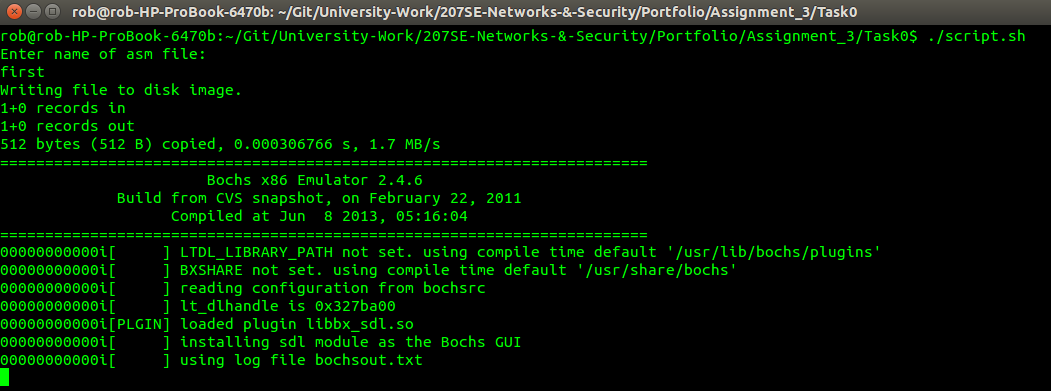
\includegraphics[width=0.9\columnwidth]{Assignment_3/Task0/e1.png}
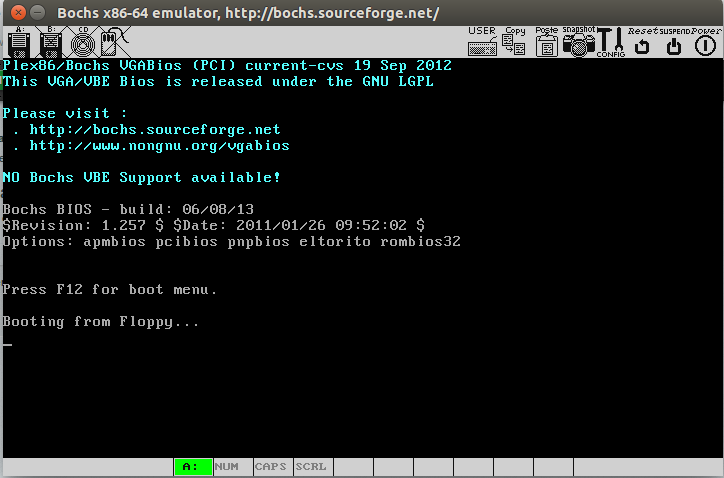
\includegraphics[width=0.9\columnwidth , height = 250px]{Assignment_3/Task0/e2.png}
\end{center}
\end{homeworkSection}
\clearpage
\begin{homeworkSection}{1. Make a Bootloader that displays my name}
\Cscript{Assignment_3/Task1/pragmalinux-img/name}{Bootloader Assembly code}
\problemAnswer{
\begin{center}
\large{Evidence of working code}\vspace{5mm}
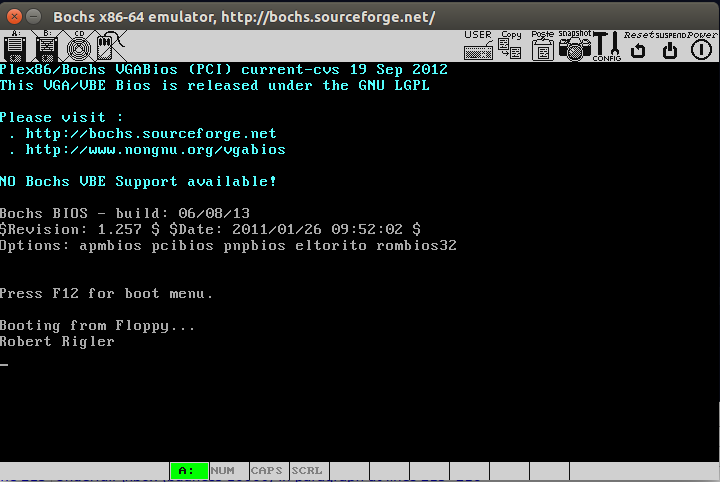
\includegraphics[width=0.9\columnwidth]{Assignment_3/Task1/pragmalinux-img/bEvi1.png}
\end{center}

\vspace{10mm}





}
\end{homeworkSection}
\begin{homeworkSection}{2. Make a Bootloader that displays a triangle of dots}
\end{homeworkSection}



\end{homeworkProblem}
\clearpage
%----------------------------------------------------------------------------------------
%	PROBLEM 4
%----------------------------------------------------------------------------------------
\begin{homeworkProblem}[Item 4 - Inside Proc]{}

\homeworkSection{1. List the CPU Information using the Cat Command}
\problemAnswer{

\begin{center}
\large{Command used \emph{: cat /proc/cpuinfo}}\vspace{3mm}
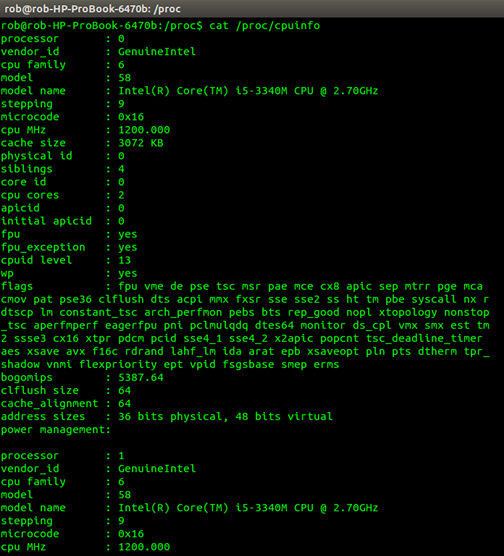
\includegraphics[width=0.75\columnwidth]{Assignment_4/1Cat.png} 
\end{center}
}

\homeworkSection{2.  Show a table of the interrupts on the system}
\problemAnswer{
\begin{center}
\large{Command used \emph{: cat /proc/interrupts}}\vspace{3mm}
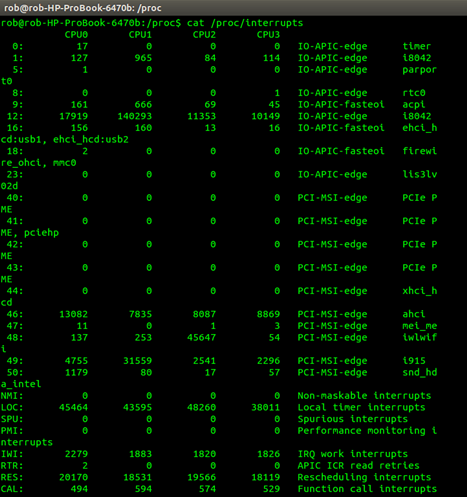
\includegraphics[width=0.75\columnwidth]{Assignment_4/2Table.png}
\end{center}
}

\homeworkSection{3.  Show number of CPUs, the producer of the CPUs and the CPU Model.}
\problemAnswer{
\begin{center}
\large{Command used \emph{: grep model /proc/cpuinfo}}\vspace{3mm}
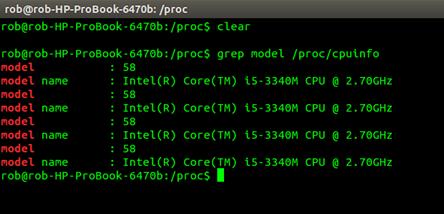
\includegraphics[width=0.75\columnwidth]{Assignment_4/3CPU.png}
\end{center}
}

\homeworkSection{4.  How the parameters that are passed to the kernel when starting up linux.}
\problemAnswer{
\begin{center}
\large{Command used \emph{: cap /proc/cmdline}}\vspace{3mm}
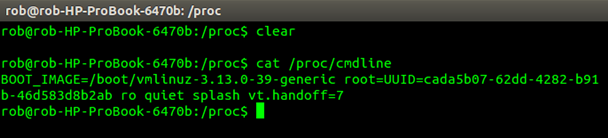
\includegraphics[width=0.75\columnwidth]{Assignment_4/4Paramaters.png}
\end{center}
}

\homeworkSection{5.  Show the name of the output devices and the number of megabytes read per second during the second sampled interval.}
\problemAnswer{

\begin{center}
\large{Command used : $awk\hspace{3mm} '\{ print\hspace{1mm} \$ 3, \$ 4 \}'\hspace{3mm} / proc/diskstats\hspace{3mm} |\hspace{3mm} grep\hspace{3mm} sda $ }\vspace{3mm}
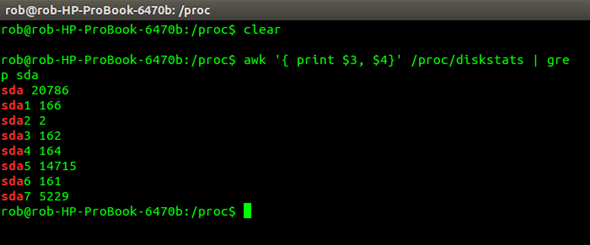
\includegraphics[width=0.75\columnwidth]{Assignment_4/5Disk.png}
\end{center}
}
\clearpage

\homeworkSection{6.  Menu based shell script.}

\Cscript{Assignment_4/BashScript}{Bash Script}


\begin{enumerate}
\clearpage
\item Output evidence of option 1: \\
\begin{center}
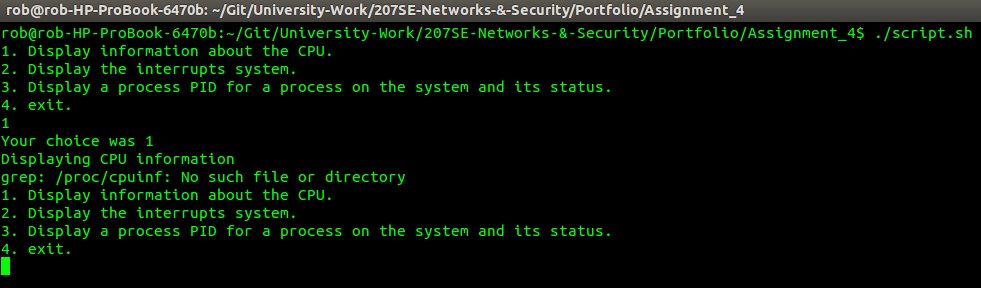
\includegraphics[width=0.9\columnwidth]{Assignment_4/s1.png}
\end{center}
\item Output evidence of option 2: \\
\begin{center}
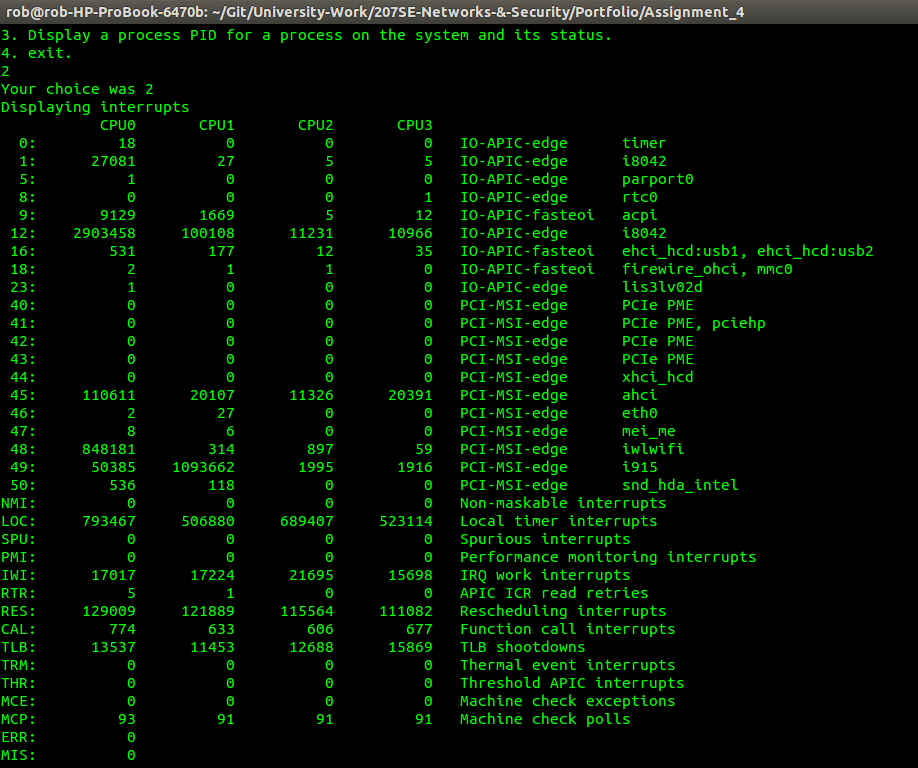
\includegraphics[width=0.9\columnwidth]{Assignment_4/s2.png}
\end{center}
\pagebreak
\item Output evidence of option 3: \\
\begin{center}
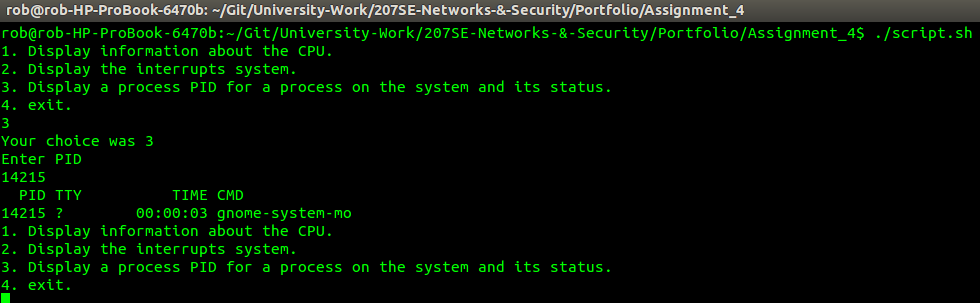
\includegraphics[width=0.9\columnwidth]{Assignment_4/s3.png}
\end{center}
\item Output evidence of option 4: \\
\begin{center}
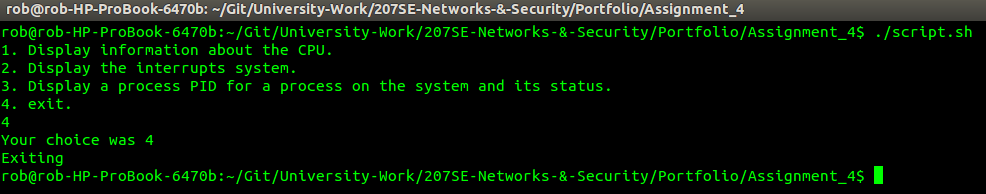
\includegraphics[width=0.9\columnwidth]{Assignment_4/s4.png}
\end{center}



\end{enumerate}

\end{homeworkProblem}
\clearpage
%----------------------------------------------------------------------------------------
%	PROBLEM 5
%----------------------------------------------------------------------------------------
\begin{homeworkProblem}[Item 5 - Buffer tutorial]{}
This task involved using buffers, specifically using buffers in term of reading an writing data from a file.
\homeworkSection{1. Commented version of the provided code}
\Cscript{Assignment_5/item1}{Commented Buffer Code}
\homeworkSection{2. Evidence of compiled code}

\problemAnswer{ 
\begin{center}
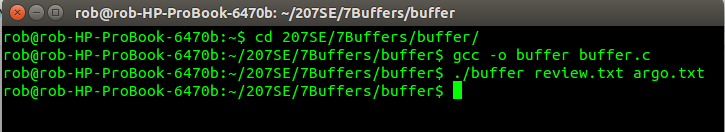
\includegraphics[width=0.75\columnwidth]{Assignment_5/2Compiled.png}\\
 
\end{center}
\large{Argo.txt contains the exact same text that was in review.txt}
}
\clearpage
\homeworkSection{3. Code adaptation to show how many characters were read in total and how many times the buffer was filled}
\Cscript{Assignment_5/item3}{Adpated Code}

Firstly I created two variables to hold the Buffer count (\emph{buf\textunderscore count}) and the character count(\emph{rd\textunderscore count})\\ (\emph{line 14}).\\Then to accumulate the total numbers of characters read  I added the value of rd\textunderscore size to the rd\textunderscore count variable (\emph{line 32})
 each time the text was read into the buffer.\\
 To count the number of times the buffer was filled, each time rd\textunderscore size was filled and its value above 0, buf\textunderscore count is incremented by 1(\emph{line 34}).
\homeworkSection{3a Evidence}
\problemAnswer{
\begin{center}
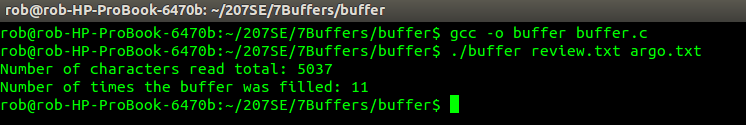
\includegraphics[width=0.9\columnwidth , height=100px]{Assignment_5/3Evidence.png}
\end{center}}
\homeworkSection{4. Altering the buffer size}
\problemAnswer{
\begin{itemize}
\item Doubling the buffer size to 1000, the program filled the buffer 6 times. This is half of the original value + 1.
\item Doubling the buffer size again to 2000 , the program filled the buffer 3 times which is half of 6.
\item Raising the the buffer size to 10000, the program filled the buffer 1 time, indicating that the entire text was placed into the buffer.
\end{itemize}
There is a direct linear correlation between the buffer size and the amount of times that the buffer was filled.

}
\clearpage

\homeworkSection{5. Adapt the code so that it is possible to compare if two files are the same.}
\Cscript{Assignment_5/item5}{Adapted code}
\homeworkSection{5a. Evidence of comparison between review.txt and argo.txt}
\problemAnswer{
\begin{center}
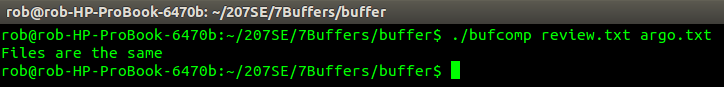
\includegraphics[width=0.9\columnwidth , height=70px]{Assignment_5/5Comp1.png}
\end{center}
}
\homeworkSection{5b. Evidence of comaprison between argo.txt and reviewobserver.txt}
\problemAnswer{
\begin{center}
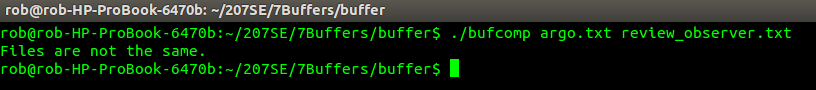
\includegraphics[width=0.9\columnwidth, height=70px]{Assignment_5/5Comp2.png}
\end{center}
}


\end{homeworkProblem}
\clearpage
%----------------------------------------------------------------------------------------
%	PROBLEM 6
%----------------------------------------------------------------------------------------
\begin{homeworkProblem}[Item 6 - Cache tutorial]{}
\homeworkSection{1. Complete the cr\textunderscore read\textunderscore byte function}
Please see the provided code in cache\textunderscore reader.c \\
\begin{enumerate}
\item Evidence of completed working code\\
\begin{center}
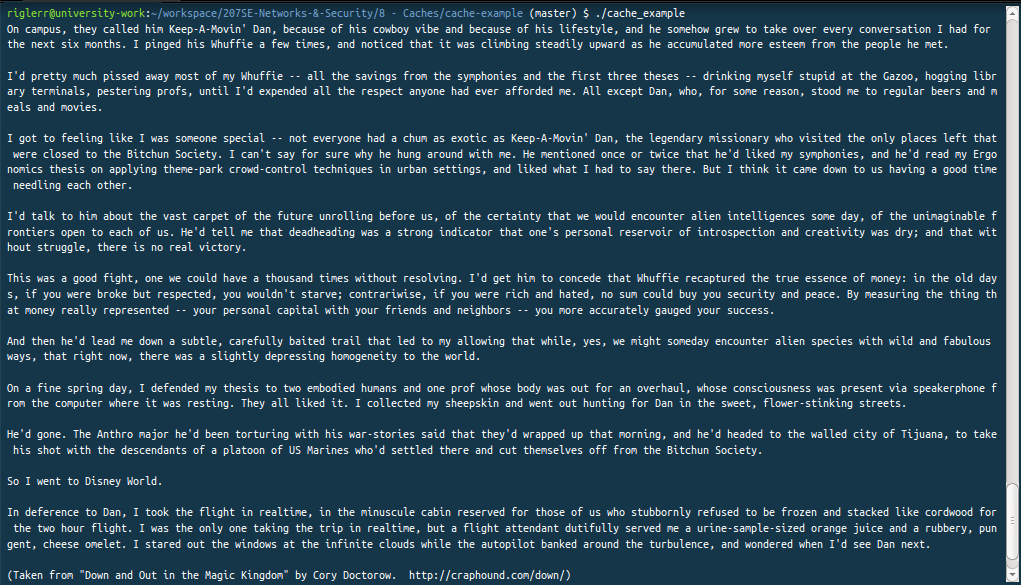
\includegraphics[width=0.9\columnwidth ]{Assignment_6/cEvi1.png}
\end{center}
\end{enumerate}
\pagebreak
\homeworkSection{2. Prove the file is being buffered}
To prove the code is being buffered. I included \emph{printf(" \textbackslash n");} on line 61 in the cache\textunderscore reader.c file . The program now starts a new line every time it reaches the end of the buffer ( in this example 20). \\

\begin{center}
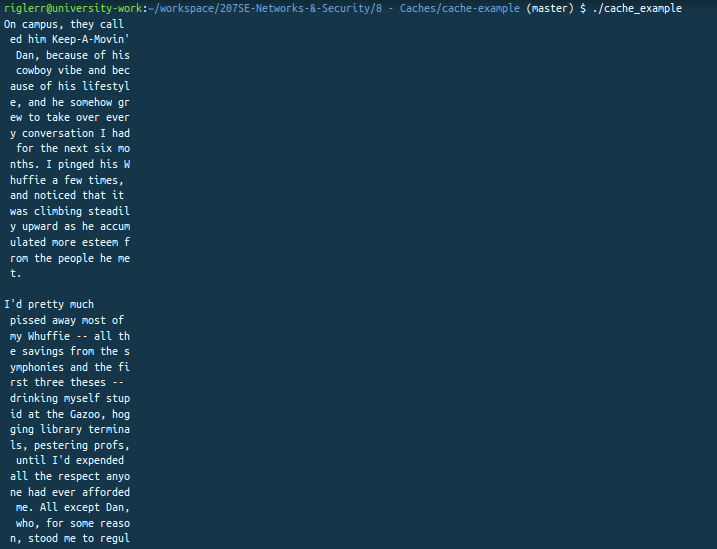
\includegraphics[width=0.9\columnwidth ]{Assignment_6/cEvi2.png}
\end{center}

\pagebreak

\homeworkSection{3. Provide some statistics}
To count the number of bytes read, I created a variable called \emph{byte\textunderscore tot} in the \emph{cr\textunderscore file}  structure (line 13) in the cache\textunderscore reader.h file. This variable is used in the \emph{Refill()} method (line 8)(\emph{cache \textunderscore reader file}). Every time the \emph{Refill()} method is called, it adds the value of \emph{len} (which contains the number of bytes currently being read) to itself.\\
The amount of times the buffer was refilled, was calculated by dividing the number of bytes read from the text by the size of the buffer.\\

\begin{enumerate}
\item Evidence of completed working code, showing the statistics: Number of bytes read and Total times the buffer was refilled.\\
\begin{center}
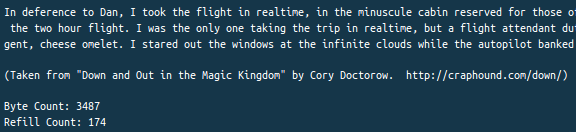
\includegraphics[width=0.9\columnwidth ]{Assignment_6/cEvi3.png}
\end{center}

\end{enumerate}
\clearpage
\Cscript{Assignment_6/cache_example}{cache\textunderscore example.c}
\clearpage

\Cscript{Assignment_6/cache_readerh}{cache\textunderscore reader.h}
\clearpage

\Cscript{Assignment_6/cache_reader}{cache\textunderscore reader.c}



\clearpage


%

\end{homeworkProblem}
\clearpage
%----------------------------------------------------------------------------------------
%	PROBLEM 7
%----------------------------------------------------------------------------------------
\begin{homeworkProblem}[Item 7 - Kernel]{}
\begin{homeworkSection}{1. Description of the commands for loading and unloading Linux kernel modules.}

\begin{itemize}
\item lsmod - Lists all of the available loaded kernel modules.
\item modinfo - Displays  information about a particular kernel module.
\item insmod - Install and load a kernel module
\item rmmod - Unload a module
\end{itemize}
\end{homeworkSection}
\begin{homeworkSection}{2. List of the loaded modules}

\large{This list was generated by using the lsmod command}
\\
\problemAnswer{
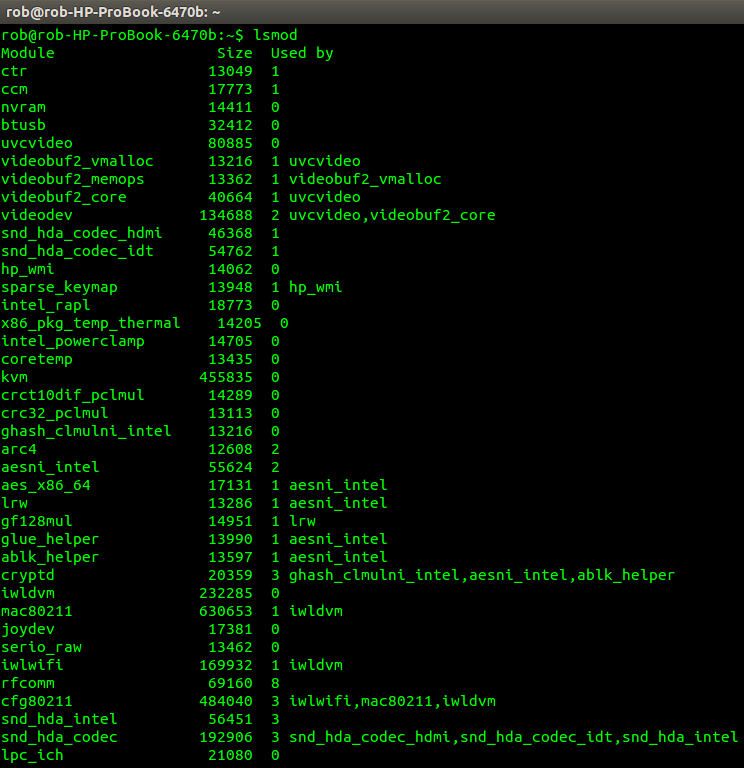
\includegraphics[width=1\columnwidth , height =400px]{Assignment_7/kEvi1.png}
}
\clearpage
\problemAnswer{
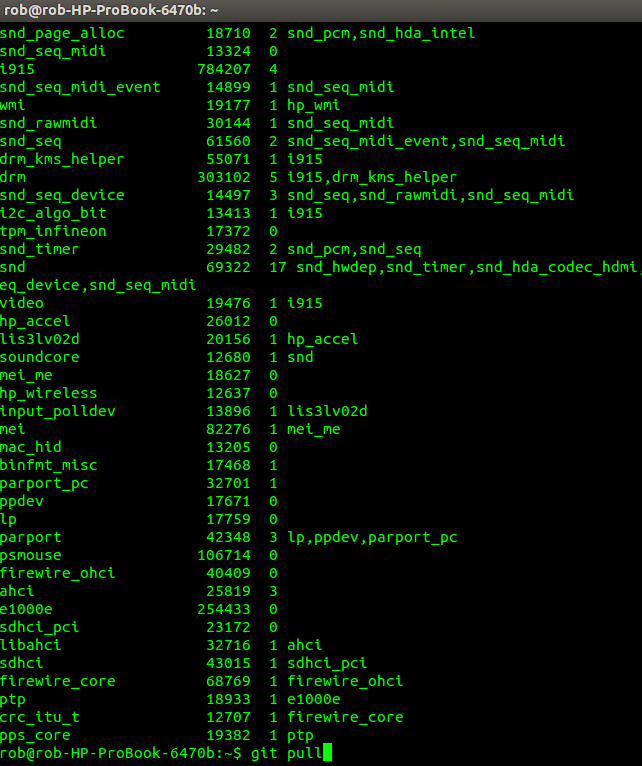
\includegraphics[width=1\columnwidth ,height =525px]{Assignment_7/kEvi2.png}}
\end{homeworkSection}
\clearpage
\begin{homeworkSection}{3. Description of four loaded modules}
\large{My selected modules are ccm, nvram, btusb, uvcvideo}

\begin{itemize}

\item \textbf{ccm}\\
	The 'ccm' module is the Clock Control Module, it controls the hardware clocks on the motherboard which consists of two crystal oscillators and a control chip. The 'ccm' ensures that the proper time is kept, so that any devices connected to the clock are using the correct time.

\item \textbf{nvram}\\
	The 'nvram' module is the Non-Volatile memory module. This driver allows the user to access the contents of the RAM in real time.
\item \textbf{btusb}\\
	The 'btusb' module is a generic Bluetooth USB driver. This driver controls the USB Bluetooth devices connected to the computer.
	
\item \textbf{uvcvideo}\\
	The 'uvcvideo' module is a UVC (USB Video Class) driver which controls webcams that are compliant to the UVC specification.
	It makes sure that the device is compatible with the video streaming functionality on the Universal-Serial-Bus.

\end{itemize}

\end{homeworkSection}{}


\pagebreak
\end{homeworkProblem}
\begin{homeworkProblem}[Item 8 - Kernel part II]{}
This task involves changing the code in cache\textunderscore reader.h and cache\textunderscore reader.c to use the kernel system calls open(), read(), and close() instead of the c alternatives fopen(), fread(), and fclose().
\begin{homeworkSection}{Changing the code}
The changes I made are:
\begin{enumerate}
\item In cache\textunderscore reader.h, in the cr\textunderscore file structure (\emph{line 7}), I changed the type of \emph{file} from: \\ FILE* \\\emph{To: }\\ int\\
This is because the system calls use integer file descriptors instead of a FILE type.
\item The line 16 of the cache\textunderscore reader.c file has been changed from:\\  int len=fread(buff-\textgreater buffer, sizeof(char), buff-\textgreater bufferlength, buff-\textgreater file);\\
 \emph{To: } \\int len=read(buff-\textgreater file,buff-\textgreater buffer, buff-\textgreater bufferlength);
\item The line 30 of the cache\textunderscore reader.c file has been changed from: \\
 fclose(f-\textgreater file);\\
  \emph{To: } \\close(f-\textgreater file);
\item The line 38 of the cache\textunderscore reader.c file has been changed from:\\
 if ((f = fopen(filename, "r")) == NULL)\\
 \emph{To: }\\ int f;\\
        f = open(filename, O\textunderscore RDONLY);\\
        if ( f \textless 0)
\end{enumerate}
\Cscript{Assignment_7/Cache/cache_reader}{cache\textunderscore reader.c}
\Cscript{Assignment_7/Cache/cache_readerh}{cache\textunderscore reader.h}
\problemAnswer{
\large{Evidence of the adapted code:}\vspace{5mm}
\begin{center}
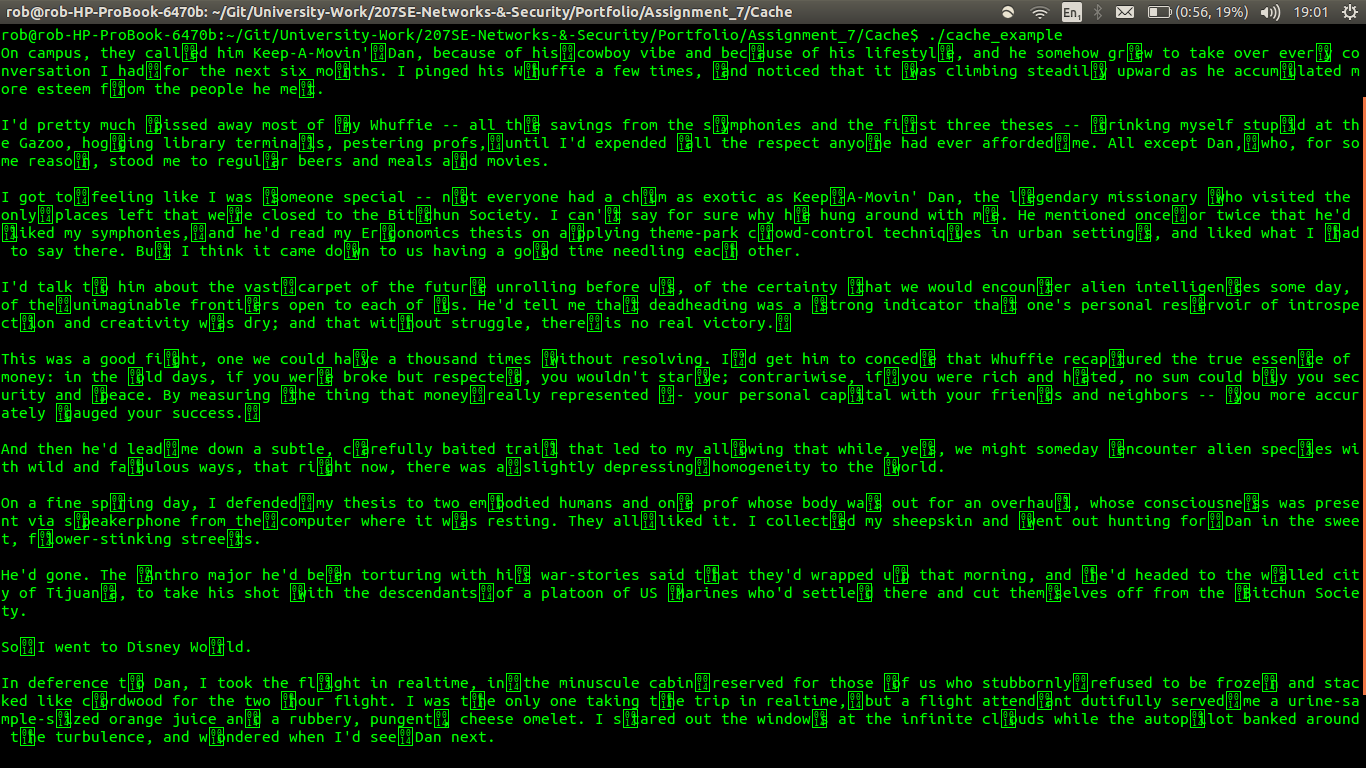
\includegraphics[width=1\columnwidth]{Assignment_7/Cache/cEvi1.png}
\vspace{5mm}

\end{center}
The output shows the contents of the file "text.txt". You may notice the strange character that appears every time the buffer is refilled.
}
\end{homeworkSection}
\end{homeworkProblem}

\end{document}